\section{Integration Testing Strategy}
The integration strategy that we are going to implement is the bottom-up approach. This choice
comes natural since we assume we already have the unit tests for the smallest
components, so we can proceed from the bottom.In this way, we will start integrating together those components that do not depend on other components to operate, or that
only depend on already developed components. The main advantages of this approach are the possibility to perform integration tests on components that are almost fully developed,to obtain feedback on how the system will react and fail in real world situations. The other advantage is that we can start testing the components following the development process,in this way we can reduce time and maximize parallelism.
Moreover, the higher-level subsystems outlined in section 2.2 are well
separated and loosely coupled since they correspond to different tiers. They
also communicate through well-defined interfaces (RESTful API), so
they will not be hard to integrate at a later time.
As we said before the \textbf{Handy Car Board},the \textbf{External System For Driving License Validation}, the \textbf{External System For Payments} and the \textbf{DBMS} are considered as black box, that have already been developed and that can be immediately used in a bottom up approach.

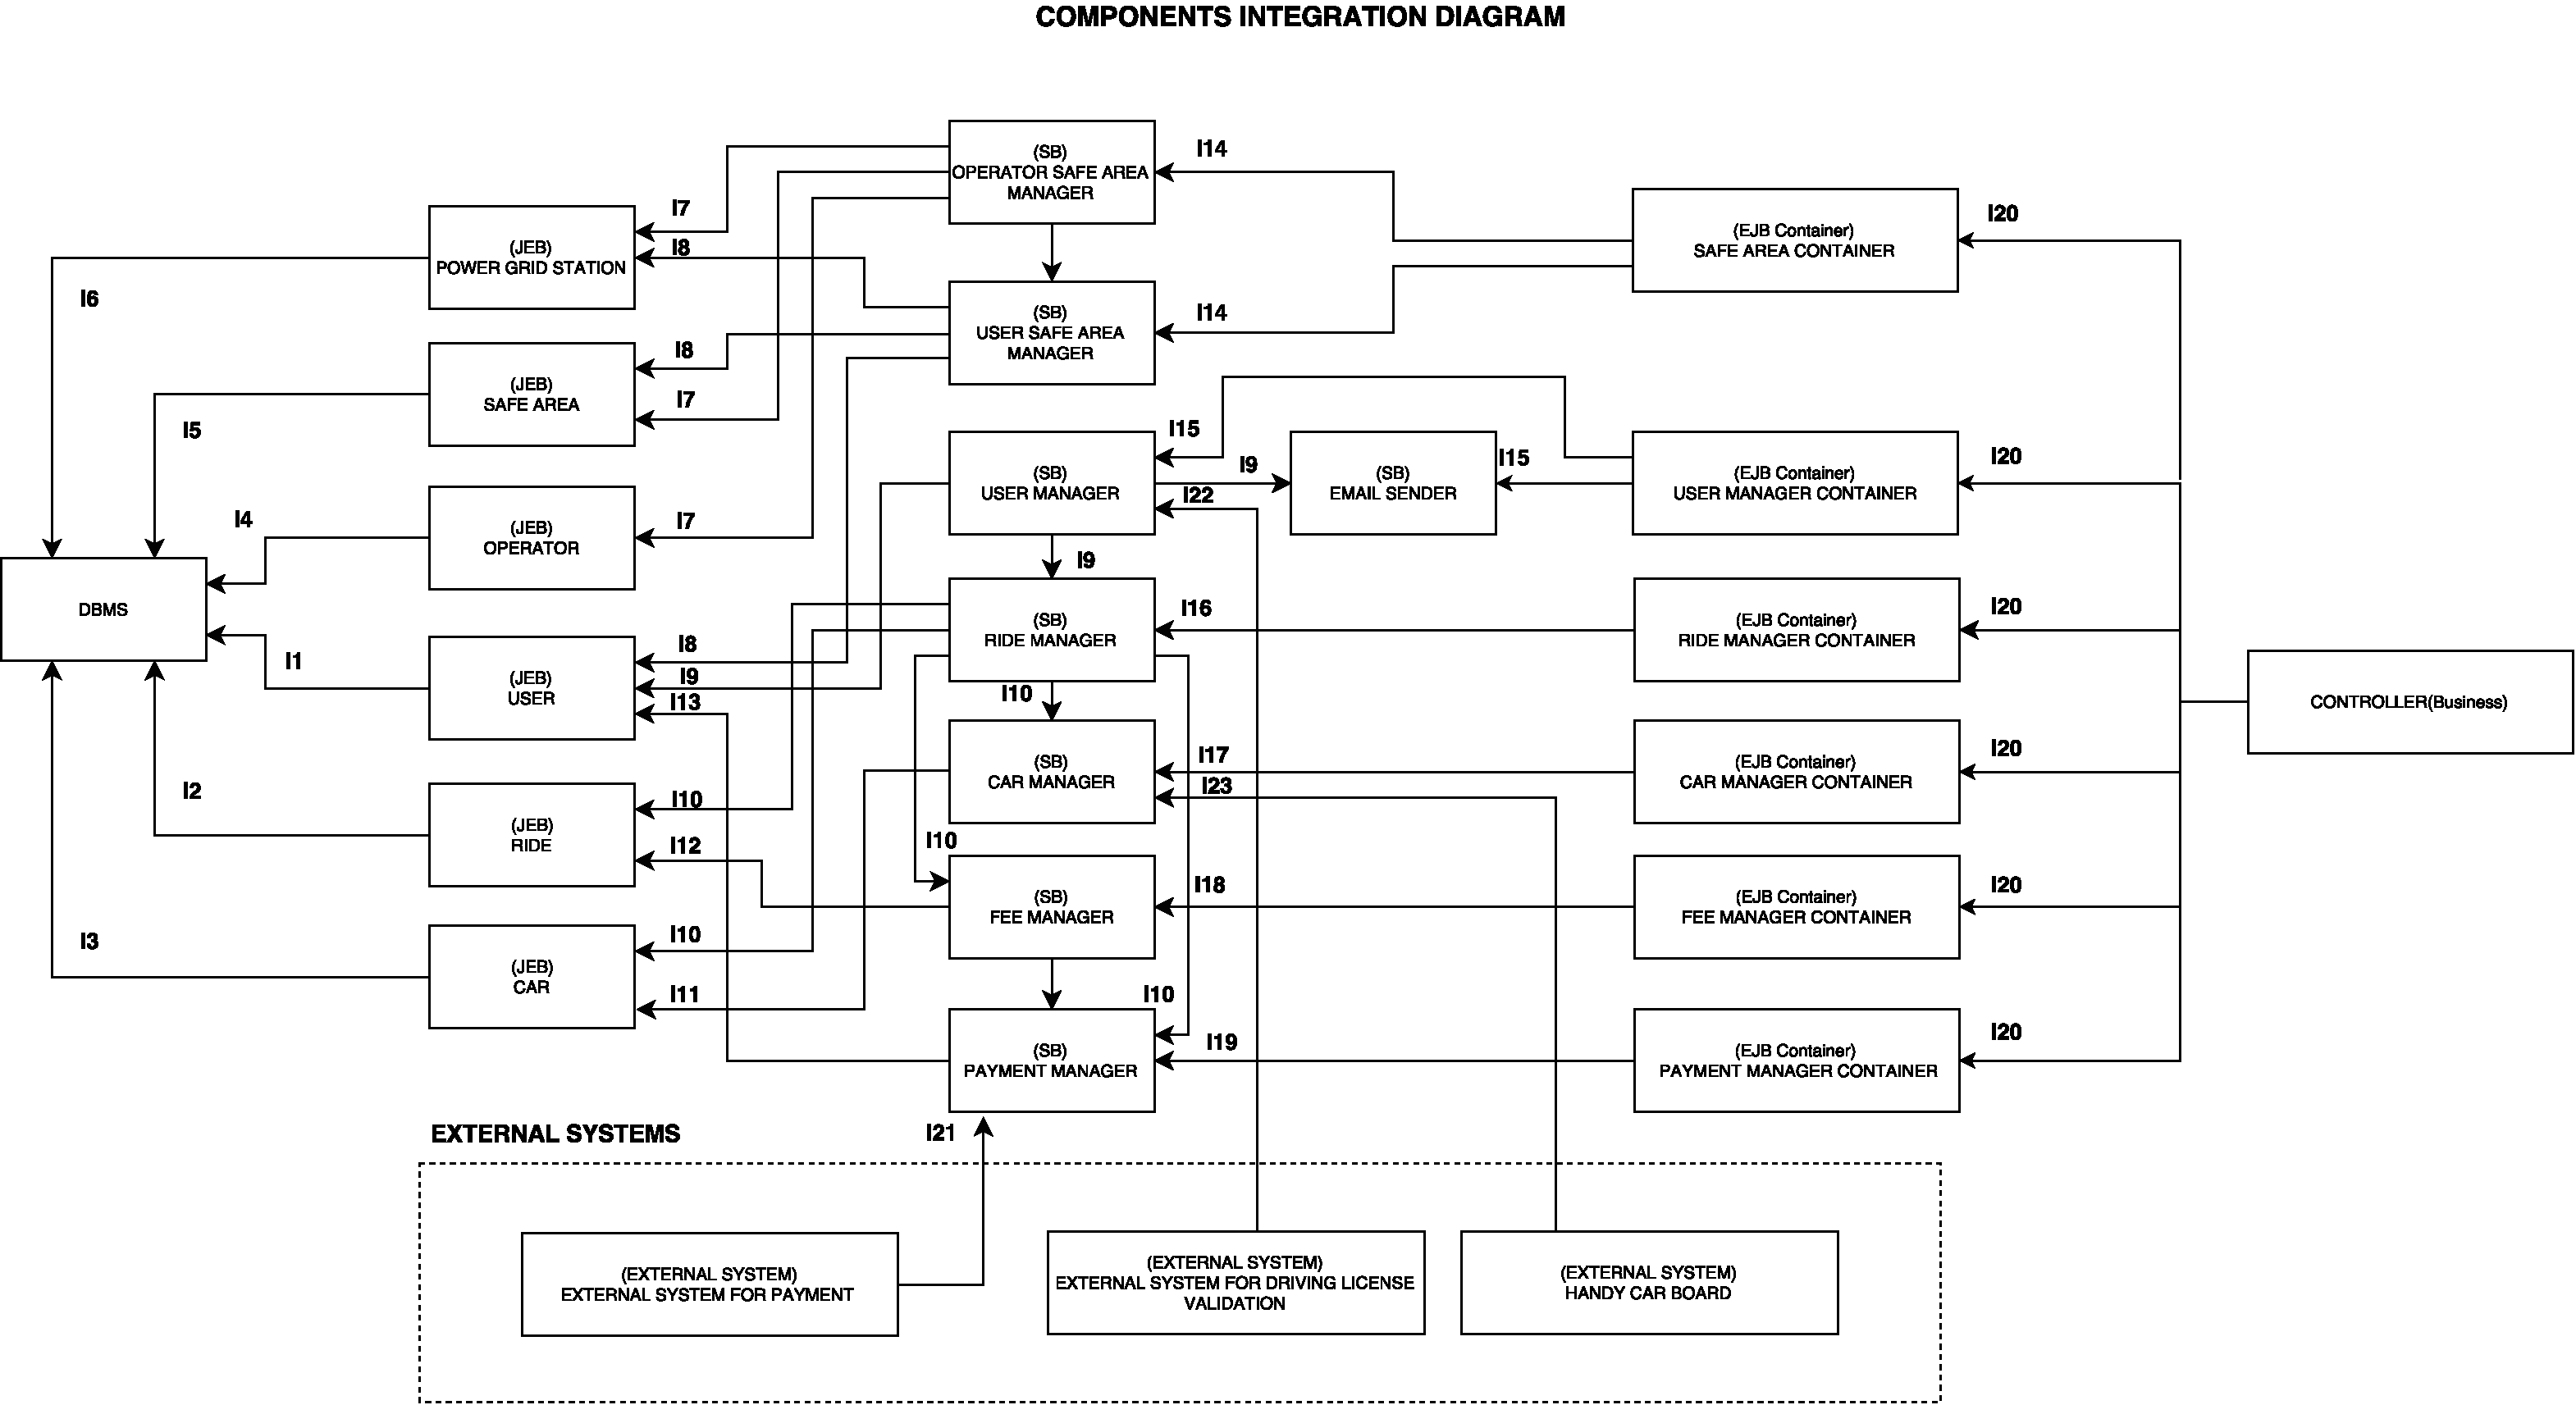
\includepdf{integration_strategy/Diagrams/IntegrationDiagram.pdf}